\documentclass{homeworg}
\usepackage{enumitem}
\usepackage{listings}
\usepackage{color} %red, green, blue, yellow, cyan, magenta, black, white
\definecolor{mygreen}{RGB}{28,172,0} % color values Red, Green, Blue
\definecolor{mylilas}{RGB}{170,55,241}
\usepackage{xcolor,cancel}
% --------------- GRAPHIC PACKAGES ----------------------------
\usepackage{graphicx}
\graphicspath{{./images/}}
\usepackage{wrapfig}
% --------------- HCANCEL COMMAND -----------------------------
\newcommand\hcancel[2][black]{\setbox0=\hbox{$#2$}%
\rlap{\raisebox{.45\ht0}{\textcolor{#1}{\rule{\wd0}{1pt}}}}#2}

% --------------- TRANSPOSE COMMAND -----------------------------
\newcommand{\transpose}[1]{\ensuremath{#1^{\scriptscriptstyle T}}}


\begin{document}

% --------------- MATLAB Code settings -----------------------
\lstset{language=Matlab,%
    %basicstyle=\color{red},
    breaklines=true,%
    morekeywords={matlab2tikz},
    keywordstyle=\color{blue},%
    morekeywords=[2]{1}, keywordstyle=[2]{\color{black}},
    identifierstyle=\color{black},%
    stringstyle=\color{mylilas},
    commentstyle=\color{mygreen},%
    showstringspaces=false,%without this there will be a symbol in the places where there is a space
    numbers=left,%
    numberstyle={\tiny \color{black}},% size of the numbers
    numbersep=9pt, % this defines how far the numbers are from the text
    emph=[1]{for,end,break},emphstyle=[1]\color{red}, %some words to emphasise
    %emph=[2]{word1,word2}, emphstyle=[2]{style},
}

% --------------- Title -------------------------------------
%\maketitle
\begin{center}
\textbf{EE 5323 - HW06}\\
\end{center}

\noindent
Bardia Mojra\\
1000766739\\
\today\\
HW06 -- Lyapunov Stability Analysis, LaSalle's Extension, and UUB\\
EE 5323 -- Nonlinear Systems\\
Dr. Frank Lewis

\exercise
\noindent
\textbf{LaSalle's Extension}\\
Consider the system from HW05,
\begin{equation*}
  \begin{cases}
    \dot{x}_1 = x_2 + x_1 (x_1^2 -2 )\\
    \dot{x}_2 = -x_1\\
  \end{cases}
\end{equation*}

We used a quadratic Lyapunov Function to show this system is locally SISL.
And we found the region within which \(\dot{V} \leq 0\).
Use LaSalle’s extension to verify that the system is AS. Find the
equilibrium point.\\
\noindent
\textbf{Answer} \\
4.a) Lyapunov function candidate: \( V(x_1, x_2) = \frac{1}{2} (x_1^2 + x_2^2) > 0\)
\begin{equation*}
\dot{V} = \frac{\partial V^\top}{\partial x} \dot{x} =
\begin{bmatrix}
\frac{\partial V}{\partial x_1} & \frac{\partial V}{\partial x_2}
\end{bmatrix}
\begin{bmatrix}
\dot{x}_1 \\
\dot{x}_2
\end{bmatrix}
=
\begin{bmatrix}
  x_1 & x_2
  \end{bmatrix}
  \begin{bmatrix}
  \dot{x}_1 \\
  \dot{x}_2
  \end{bmatrix}
  \Rightarrow
\end{equation*}
\begin{equation*}
\dot{V} =
  x_1 \dot{x}_1 + x_2 \dot{x}_2
\end{equation*}
Now we plug in system dynamics to check stability,
\begin{equation*}
  \dot{V} = x_1 (x_2 + x_1 (x_1^2 -2)) + x_2(-x_1) \Rightarrow
\end{equation*}
\begin{equation*}
  \dot{V} = \hcancel[red]{x_1 x_2} - x_1^2(x_1^2 -2) - \hcancel[red]{x_1 x_2}
\end{equation*}
\begin{equation*}
  \dot{V} = - x_1^2(x_1^2 -2) \leq 0
\end{equation*}
Thus, the system is \emph{asymptotically stable} (AS) and it is bound by a region
with radius of \(\sqrt{2}\). Moreover, we know \(\dot{x} \rightarrow 0\); thus,
per LaSalle’s extension, \(\ddot{x} \rightarrow 0\) must hold true (not used in
system dynamics). We proceed with plugging in the resulting \(x_1\) in the
system dynamics equation.
\begin{equation*}
  \dot{V} = - x_1^2(x_1^2 -2) \leq 0 \Rightarrow \dot{V} \rightarrow 0,~x_1~|~x_{1}^{2} - 2 = 0; \Rightarrow x_1 = \pm sqrt{2}
\end{equation*}
\begin{equation*}
  \begin{cases}
    \dot{x}_1 = x_2 + x_1 (x_1^2 -2 )\\
    \dot{x}_2 = -x_1\\
  \end{cases}
\end{equation*}





4.b) Simulation:
\begin{figure}[h]
  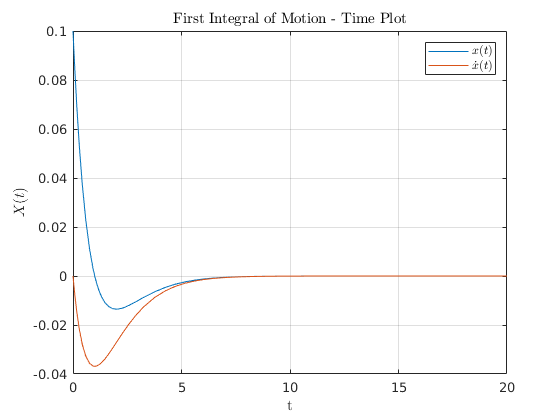
\includegraphics[width=.6\textwidth]{fig01.png}
  \centering
\end{figure}
\begin{figure}[h]
  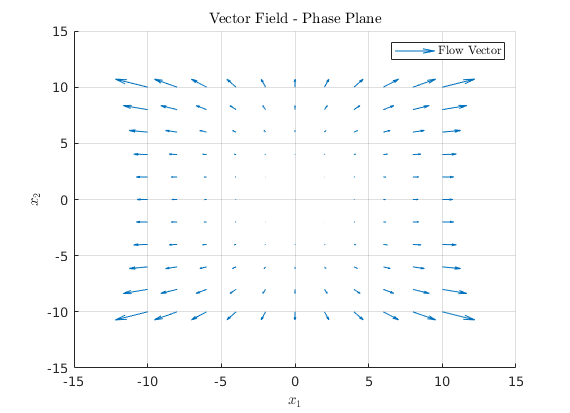
\includegraphics[width=.6\textwidth]{fig02.png}
  \centering
\end{figure}
\begin{figure}[h]
  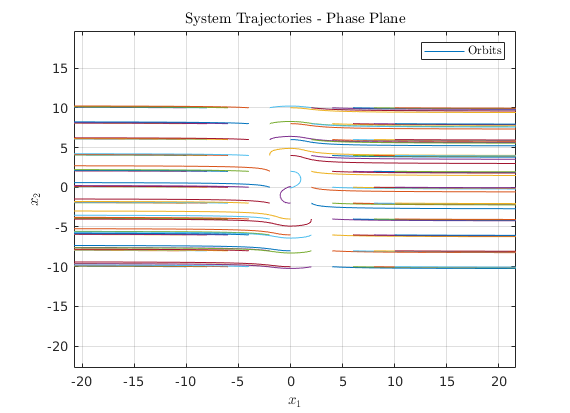
\includegraphics[width=.6\textwidth]{fig03.png}
  \centering
\end{figure}

\newpage
\newpage
\newpage

\noindent
\textbf{Matlab Code}
\lstinputlisting{../q01_main.m}
\lstinputlisting{../q01_sys.m}




\exercise
\noindent
\textbf{Limit Cycles}\\
Consider the following system,
\begin{equation*}
  \begin{cases}
    \dot{x} = 4 x^2 y - f_1 (x) \left( x^2 + 2 y^2 -4  \right)\\
    \dot{y} = 2 x^3 - f_1 (y) \left( x^2 + 2 y^2 -4  \right)\\
  \end{cases}
\end{equation*}

where the continuous functions \(f_1 (x)\), \(f_2 (y)\) have the same sign as
their argument. Show that the system tends towards a limit cycle independent of the explicit expressions of \(f_1 (x)\), \(f_2 (y)\).\\

\noindent
\textbf{Answer} \\



\exercise
\noindent
\textbf{UUB of a System with Disturbance}\\
Consider the system on S\&L p. 66 with a disturbance d,
\begin{equation*}
  \dot{x} + c(x) + d = 0
\end{equation*}
Assume that \(xc(x) a x^2 \) with \( a > 0\) a known positive constant.\\
a. Assume that d is unknown but is bounded by \(||d|| < D \) with D a known positive constant. Prove that the system is UUB and find the bound on \(x(t)\).\\
b. Assume that d is unknown but is bounded by \(||d|| < D||x|| \) with D a known positive constant. Prove that the system is UUB and find the bound on \(x(t)\).\\

\noindent
\textbf{Answer} \\

\exercise
\noindent
\textbf{Lyapunov Analysis}\\
Use Lyapunov Equation to check the stability of the linear systems.

a. \( \dot{x} = Ax = \begin{bmatrix}
  0 & 1\\
  -6 & -5\\
\end{bmatrix} x \)

b. \( \dot{x} = Ax = \begin{bmatrix}
  -7 & 4\\
  -7 & 3\\
\end{bmatrix} x \)

c. \( \dot{x} = Ax = \begin{bmatrix}
   0 & 1\\
  -4 & 0\\
\end{bmatrix} x \)

\noindent
\textbf{Answer} \\



\end{document}
